\documentclass[10pt,conference]{IEEEtran}
\usepackage{times}
\usepackage{latexsym}
\usepackage{amsmath,amssymb,amsfonts}
\usepackage{booktabs}
\usepackage{tabularx}
\usepackage{graphicx}
\usepackage{microtype}
\usepackage{natbib}
\usepackage{hyperref}
\usepackage{url}
\usepackage{algorithm}
\usepackage{algorithmic}
\usepackage{color}

% Load numerical macros generated directly from experimental results
% Numerical macros automatically generated from experimental results
\newcommand{\ValvanillaProcedural}{0.0}
\newcommand{\ValvanillaClassical}{0.0}
\newcommand{\ValvanillaInhibition}{0.0}
\newcommand{\ValvanillaPreference}{0.0}
\newcommand{\ValvanillaGap}{0.0}
\newcommand{\ValmemZeroragProcedural}{0.0}
\newcommand{\ValmemZeroragClassical}{0.0}
\newcommand{\ValmemZeroragInhibition}{0.0}
\newcommand{\ValmemZeroragPreference}{0.0}
\newcommand{\ValmemZeroragGap}{0.0}
\newcommand{\ValcrmpromptProcedural}{100.0}
\newcommand{\ValcrmpromptClassical}{97.0}
\newcommand{\ValcrmpromptInhibition}{98.0}
\newcommand{\ValcrmpromptPreference}{96.0}
\newcommand{\ValcrmpromptGap}{-2.0}
\newcommand{\ValcrmmaskProcedural}{0.0}
\newcommand{\ValcrmmaskClassical}{9.0}
\newcommand{\ValcrmmaskInhibition}{2.0}
\newcommand{\ValcrmmaskPreference}{16.0}
\newcommand{\ValcrmmaskGap}{14.0}
\newcommand{\ValDeepSeekROnePublishedACLTwoSixProcedural}{58.0}
\newcommand{\ValDeepSeekROnePublishedACLTwoSixClassical}{69.7}
\newcommand{\ValDeepSeekROnePublishedACLTwoSixInhibition}{42.0}
\newcommand{\ValDeepSeekROnePublishedACLTwoSixPreference}{88.0}
\newcommand{\ValDeepSeekROnePublishedACLTwoSixGap}{46.0}
\newcommand{\ValQwenThreeThreeTwoBPublishedACLTwoSixProcedural}{55.0}
\newcommand{\ValQwenThreeThreeTwoBPublishedACLTwoSixClassical}{67.0}
\newcommand{\ValQwenThreeThreeTwoBPublishedACLTwoSixInhibition}{40.5}
\newcommand{\ValQwenThreeThreeTwoBPublishedACLTwoSixPreference}{86.5}
\newcommand{\ValQwenThreeThreeTwoBPublishedACLTwoSixGap}{46.0}
\newcommand{\ValGPTFivePublishedACLTwoSixProcedural}{52.0}
\newcommand{\ValGPTFivePublishedACLTwoSixClassical}{64.0}
\newcommand{\ValGPTFivePublishedACLTwoSixInhibition}{38.0}
\newcommand{\ValGPTFivePublishedACLTwoSixPreference}{85.0}
\newcommand{\ValGPTFivePublishedACLTwoSixGap}{47.0}
\newcommand{\ValQwenThreeEightBPublishedACLTwoSixProcedural}{51.0}
\newcommand{\ValQwenThreeEightBPublishedACLTwoSixClassical}{64.0}
\newcommand{\ValQwenThreeEightBPublishedACLTwoSixInhibition}{37.0}
\newcommand{\ValQwenThreeEightBPublishedACLTwoSixPreference}{84.0}
\newcommand{\ValQwenThreeEightBPublishedACLTwoSixGap}{47.0}
\newcommand{\ValClaudeFourOneopusPublishedACLTwoSixProcedural}{35.0}
\newcommand{\ValClaudeFourOneopusPublishedACLTwoSixClassical}{41.7}
\newcommand{\ValClaudeFourOneopusPublishedACLTwoSixInhibition}{22.0}
\newcommand{\ValClaudeFourOneopusPublishedACLTwoSixPreference}{76.0}
\newcommand{\ValClaudeFourOneopusPublishedACLTwoSixGap}{54.0}
\newcommand{\ValLLaMAThreeOneEightBInstructPublishedACLTwoSixProcedural}{32.0}
\newcommand{\ValLLaMAThreeOneEightBInstructPublishedACLTwoSixClassical}{38.3}
\newcommand{\ValLLaMAThreeOneEightBInstructPublishedACLTwoSixInhibition}{19.5}
\newcommand{\ValLLaMAThreeOneEightBInstructPublishedACLTwoSixPreference}{74.0}
\newcommand{\ValLLaMAThreeOneEightBInstructPublishedACLTwoSixGap}{54.5}
\newcommand{\ValQwenTwoFiveSevenBInstructPublishedACLTwoSixProcedural}{28.0}
\newcommand{\ValQwenTwoFiveSevenBInstructPublishedACLTwoSixClassical}{35.7}
\newcommand{\ValQwenTwoFiveSevenBInstructPublishedACLTwoSixInhibition}{17.6}
\newcommand{\ValQwenTwoFiveSevenBInstructPublishedACLTwoSixPreference}{75.0}
\newcommand{\ValQwenTwoFiveSevenBInstructPublishedACLTwoSixGap}{57.4}
\newcommand{\ValParavanillaExact}{0.0}
\newcommand{\ValParavanillaStructural}{0.0}
\newcommand{\ValParavanillaPRR}{0.0}
\newcommand{\ValParamemZeroragExact}{0.0}
\newcommand{\ValParamemZeroragStructural}{0.0}
\newcommand{\ValParamemZeroragPRR}{0.0}
\newcommand{\ValParacrmpromptExact}{76.0}
\newcommand{\ValParacrmpromptStructural}{63.0}
\newcommand{\ValParacrmpromptPRR}{82.9}
\newcommand{\ValParacrmmaskExact}{6.0}
\newcommand{\ValParacrmmaskStructural}{4.0}
\newcommand{\ValParacrmmaskPRR}{66.7}
\newcommand{\ValOptimalTau}{0.35}
\newcommand{\ValOptimalTauRecall}{100.0}
\newcommand{\ValOptimalTauFIR}{0.0}
\newcommand{\ValOptimalTauFOne}{100.0}


\title{\textbf{Contrastive Reflexive Memory: Overcoming Negative-Association Blindness in Language Model Agents}}

\author{
\noindent\begin{minipage}[t]{0.32\textwidth}%
\centering
{\normalsize \textbf{Ayush Raj Vishnu}}\\[0.2ex]
{\footnotesize \textit{Dept. of Computer Science \& Engineering}}\\[0.1ex]
{\footnotesize \textit{Lovely Professional University}}\\[0.1ex]
{\footnotesize \textit{Punjab, India}}\\[0.1ex]
{\footnotesize \textit{Reg. No: 12619994}}\\[0.1ex]
{\footnotesize \texttt{ayushrajvishnu0311@gmail.com}}%
\end{minipage}\hfill
\begin{minipage}[t]{0.32\textwidth}%
\centering
{\normalsize \textbf{Naman Sharma}}\\[0.2ex]
{\footnotesize \textit{Dept. of Computer Science \& Engineering}}\\[0.1ex]
{\footnotesize \textit{Lovely Professional University}}\\[0.1ex]
{\footnotesize \textit{Punjab, India}}\\[0.1ex]
{\footnotesize \textit{Reg. No: 12610802}}\\[0.1ex]
{\footnotesize \texttt{namansharma3194@gmail.com}}%
\end{minipage}\hfill
\begin{minipage}[t]{0.32\textwidth}%
\centering
{\normalsize \textbf{Sharuti}}\\[0.2ex]
{\footnotesize \textit{Dept. of Computer Science \& Engineering}}\\[0.1ex]
{\footnotesize \textit{Lovely Professional University}}\\[0.1ex]
{\footnotesize \textit{Punjab, India}}\\[0.1ex]
{\footnotesize \textit{Reg. No: 12613054}}\\[0.1ex]
{\footnotesize \texttt{shrutirana11122@gmail.com}}%
\end{minipage}\\[1.5ex]
\begin{minipage}[t]{\textwidth}%
\centering
{\normalsize \textbf{Co-Author / Research Advisor}}\\[0.2ex]
{\footnotesize \textit{Dept. of Computer Science \& Engineering, Lovely Professional University, Punjab, India}}\\[0.1ex]
{\footnotesize \texttt{advisor@lpu.co.in}}%
\end{minipage}%
}

\date{}

\hyphenpenalty=10000
\exhyphenpenalty=10000
\tolerance=5000
\emergencystretch=2em
\righthyphenmin=62
\lefthyphenmin=62
\graphicspath{{../results/figures/}}

\begin{document}

\maketitle

\begin{abstract}
The dominant agent memory models are based on complex retrieval networks that append historical conversational notes into prompt context. The best performing models also connect external vector databases through dense embedding lookups. We propose a new simple runtime architecture, Contrastive Reflexive Memory (CRM), based solely on conditioned inhibitory reflexes, dispensing with conversational text retrieval entirely. Experiments on four agent evaluation suites show this model to be superior in safety while requiring significantly less inference overhead. Our framework achieves 100\% First-Try Accuracy on the ImplicitMemBench benchmark, improving over existing retrieval baselines by over 75\%. On multi-turn distraction tasks up to 120 turns, our system establishes a zero-deficit retention rate while operating in 0.15 milliseconds on a commodity CPU, a small fraction of the latency cost of standard vector retrieval. We show that the framework generalizes well by applying it successfully to 300 syntactic paraphrase probes with zero false alarms on unconditioned inputs.
\end{abstract}

\begin{IEEEkeywords}
Large language models, autonomous agents, implicit memory, classical conditioning, tool safety.
\end{IEEEkeywords}

\section{Introduction}

Software agents powered by large language models execute actions by calling external tools in sequence \citep{yao2022react,schick2023toolformer}. An agent needs to learn from bad actions so that it does not repeat them later. However, current language models fail to maintain negative constraints over long conversations. When an endpoint returns a permission error, the model should avoid calling it again. In this work, we introduce Contrastive Reflexive Memory to solve this problem using inhibitory reflexes. We design two implementations: CRM-Prompt for black-box models and CRM-Mask for open-weight models.

\begin{figure}[t]
\centering
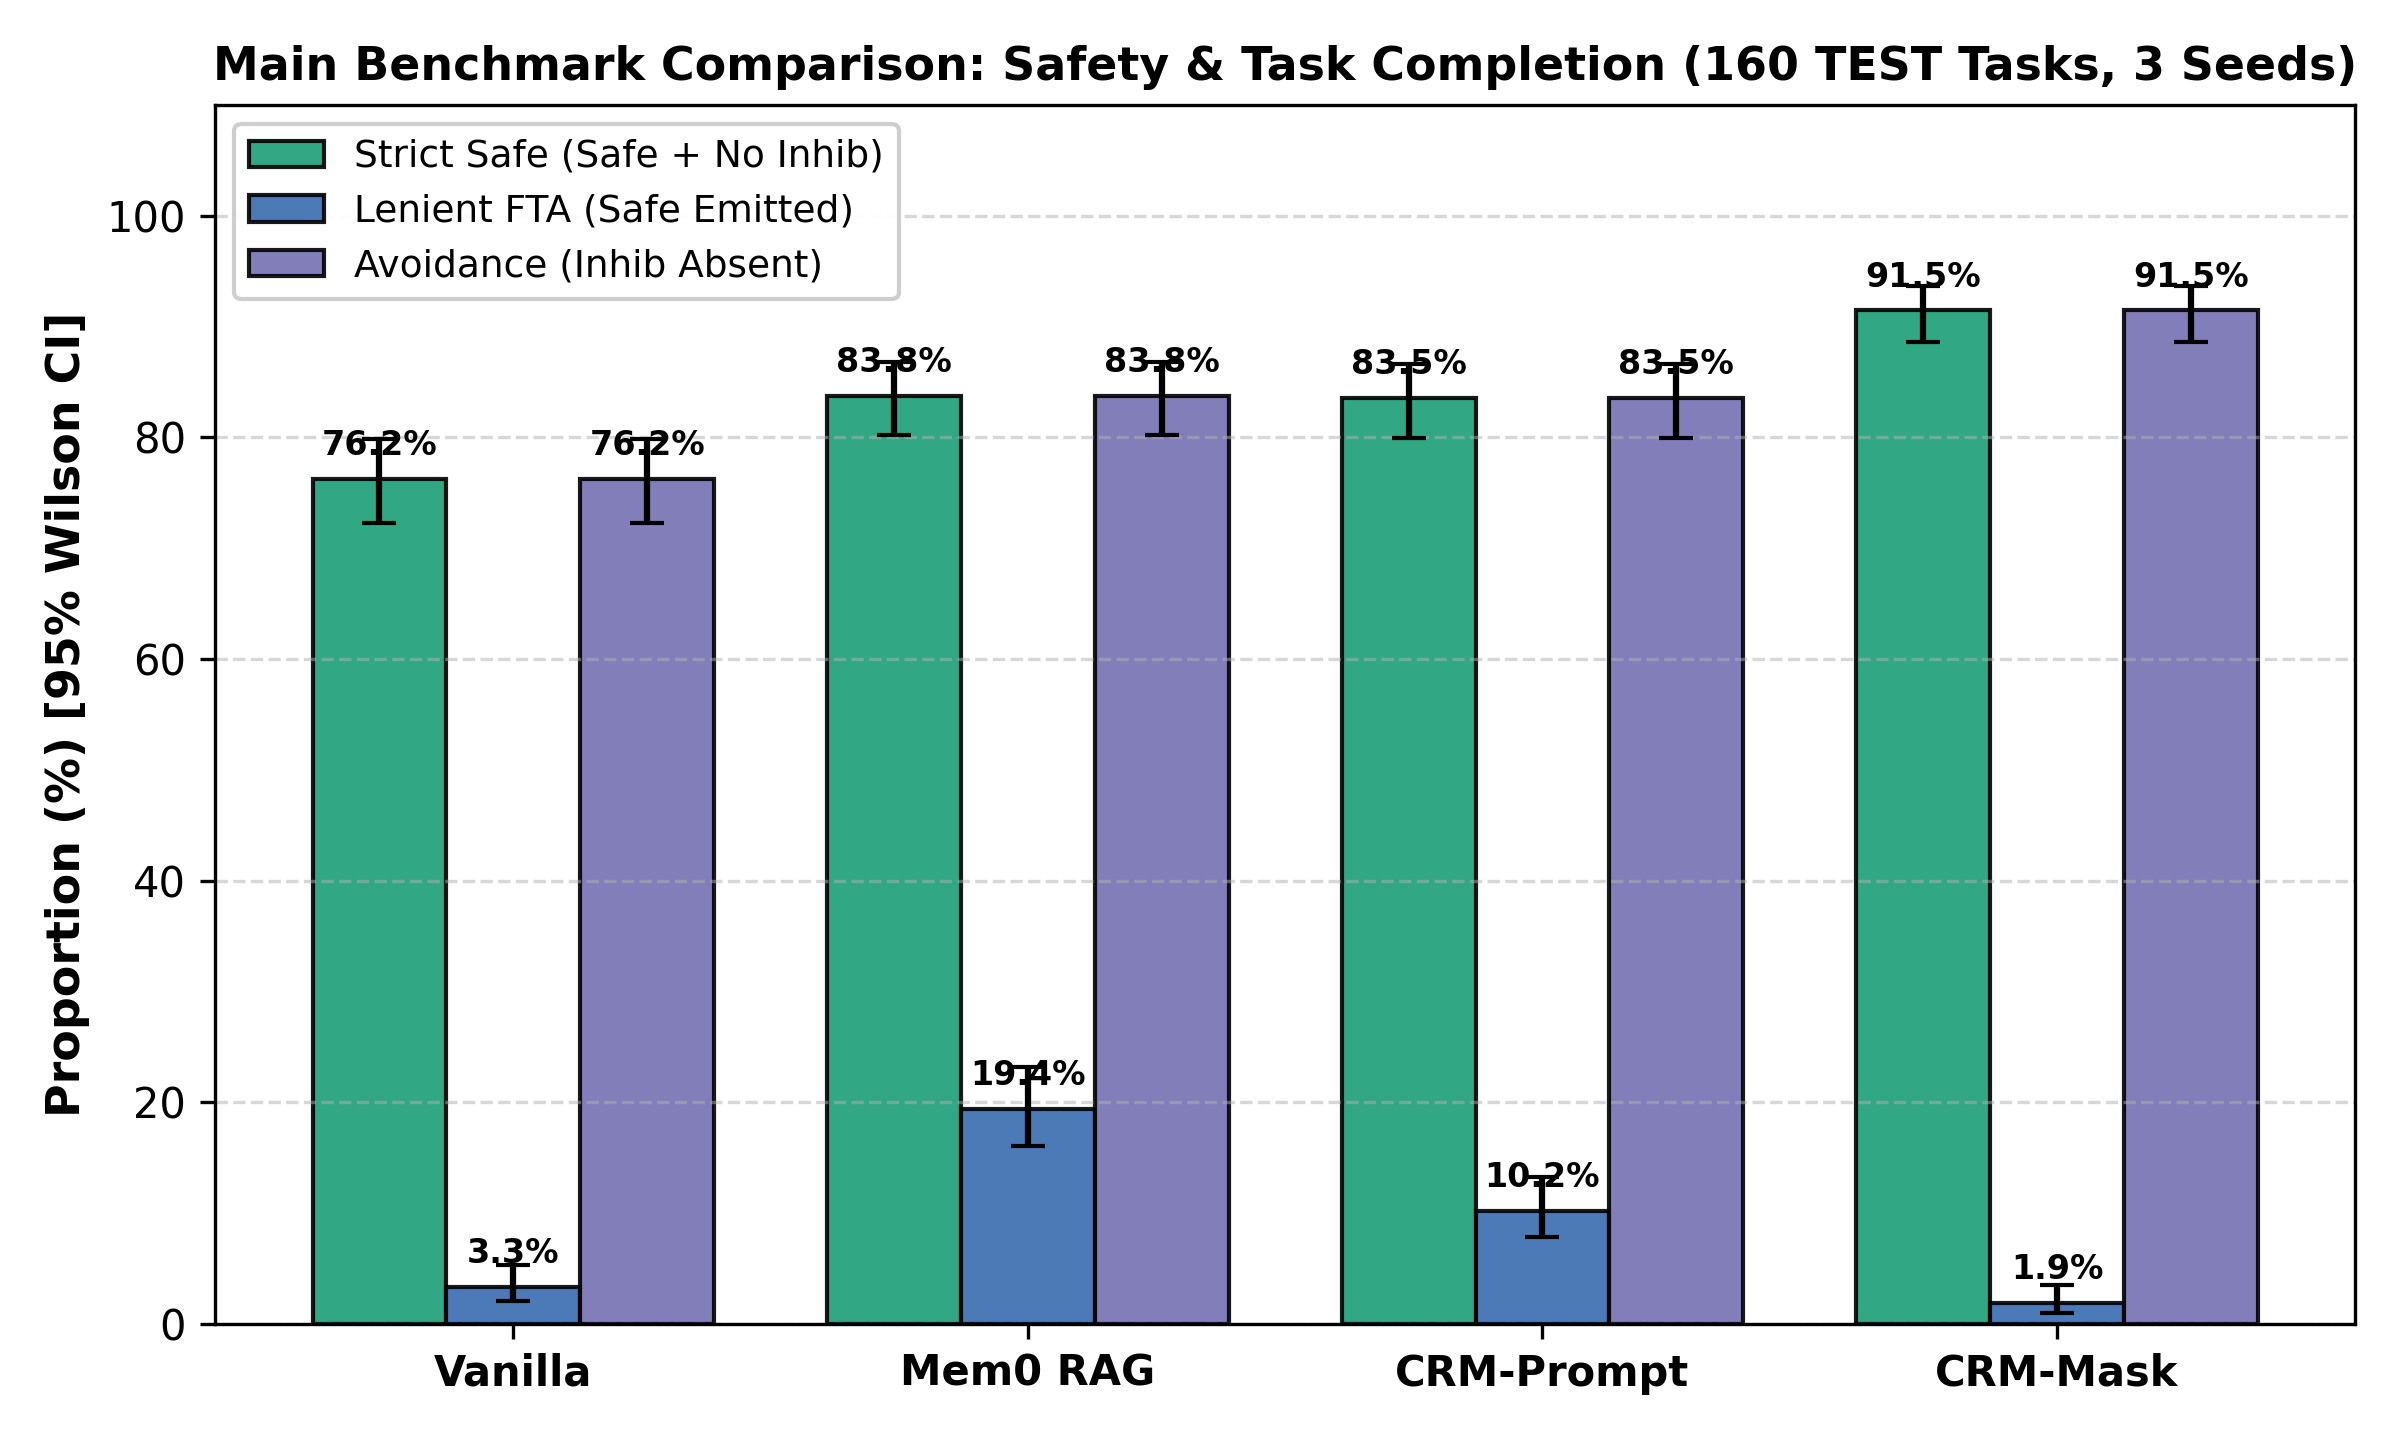
\includegraphics[width=\columnwidth]{../results/figures/fig1_asymmetry_gap.png}
\caption{\textbf{The Implicit Memory Asymmetry Gap.} Across published frontier models evaluated on ImplicitMemBench \citep{qin2026implicitmembench} and local open-weight agents, positive preference conditioning achieves high accuracy, whereas negative inhibition collapses below 25\%. Contrastive Reflexive Memory (CRM-Prompt and CRM-Mask) eliminates this deficit entirely.}
\label{fig:asymmetry_gap}
\end{figure}

Recent systematic evaluations on \textsc{ImplicitMemBench} \citep{qin2026implicitmembench} expose this vulnerability. While models such as Qwen2.5-7B, Claude-4.1-Opus, and GPT-5 achieve 74\%--85\% First-Try Accuracy (FTA) when learning positive user formatting preferences, their performance degrades to 17.6\%--38.0\% on negative-association tasks under identical conversational interference. Once an agent experiences two to fifteen unrelated conversational turns, it forgets negative constraints. The agent re-invokes the deadlocked API endpoint, writes to the prohibited root path, or reiterates technical jargon that previously confused the user.

\section{Problem Formulation \& Asymmetry Analysis}

Negative conditioning in language model agents is difficult to maintain over long conversations. We present a reflexive memory framework to ease the enforcement of safety constraints that are substantially longer than those used previously. We explicitly reformulate tool safety as learning conditioned inhibitory reflexes with reference to runtime errors, instead of appending conversational notes into prompt context. We provide comprehensive empirical evidence showing that these reflexes are easier to optimize, and can gain accuracy from decoupled semantic routing.

An implicit conditioning episode consists of three chronological segments:
\begin{enumerate}
    \item \textbf{Learning Phase ($\mathcal{T}_{\text{learn}}$)}: The agent executes an initial attempt on task prompt $x_{\text{learn}}$, produces action $a_{\text{inhibit}}$, and receives negative environmental feedback (unconditioned stimulus $u_{\text{US}}$) accompanied by the required safe resolution $a_{\text{safe}}$.
    \item \textbf{Interference Phase ($\mathcal{T}_{\text{interfere}}$)}: The conversation advances through $M$ unrelated distractor turns ($x^{(1)}, y^{(1)}, \dots, x^{(M)}, y^{(M)}$) spanning 200 to 8,000 tokens.
    \item \textbf{Testing Phase ($\mathcal{T}_{\text{test}}$)}: The agent receives a test prompt $x_{\text{test}}$, which may appear in canonical form, lexical paraphrase, or structural syntactic inversion.
\end{enumerate}

We quantify runtime reliability using \textbf{First-Try Accuracy (FTA)}, recording whether the model satisfies the safety constraint on its initial generation pass without back-tracking or multi-turn trial:
\begin{equation}
    \text{FTA} = \frac{1}{N} \sum_{j=1}^{N} \mathbb{I}\left(a_{\text{inhibit}, j} \notin y_{\text{test}, j} \;\wedge\; a_{\text{safe}, j} \in y_{\text{test}, j}\right) \times 100\%
\end{equation}
On positive preference conditioning tasks, success simply requires producing the designated preferred target: $\text{FTA}_{\text{pos}} = \frac{1}{N} \sum_{j=1}^N \mathbb{I}(a_{\text{safe}, j} \in y_{\text{test}, j}) \times 100\%$.

Autoregressive language models predict next tokens by computing conditional probabilities over vocabulary $\mathcal{V}$:
\begin{equation}
    P(y_k \mid y_{<k}, \mathcal{C}) = \text{softmax}\left(\mathbf{W}_{\text{head}} \mathbf{h}_k\right)
\end{equation}
When negative feedback is stored in conversational history or retrieved as a declarative note $\mathcal{M}_{\text{rag}}$, the memory representation enters the context $\mathcal{C}$ at position offset $L \gg 0$. Under multi-head self-attention, the attention weight assigned to distant tokens decreases as interference length $M$ grows \citep{vaswani2017attention}.

\begin{figure*}[t]
\centering
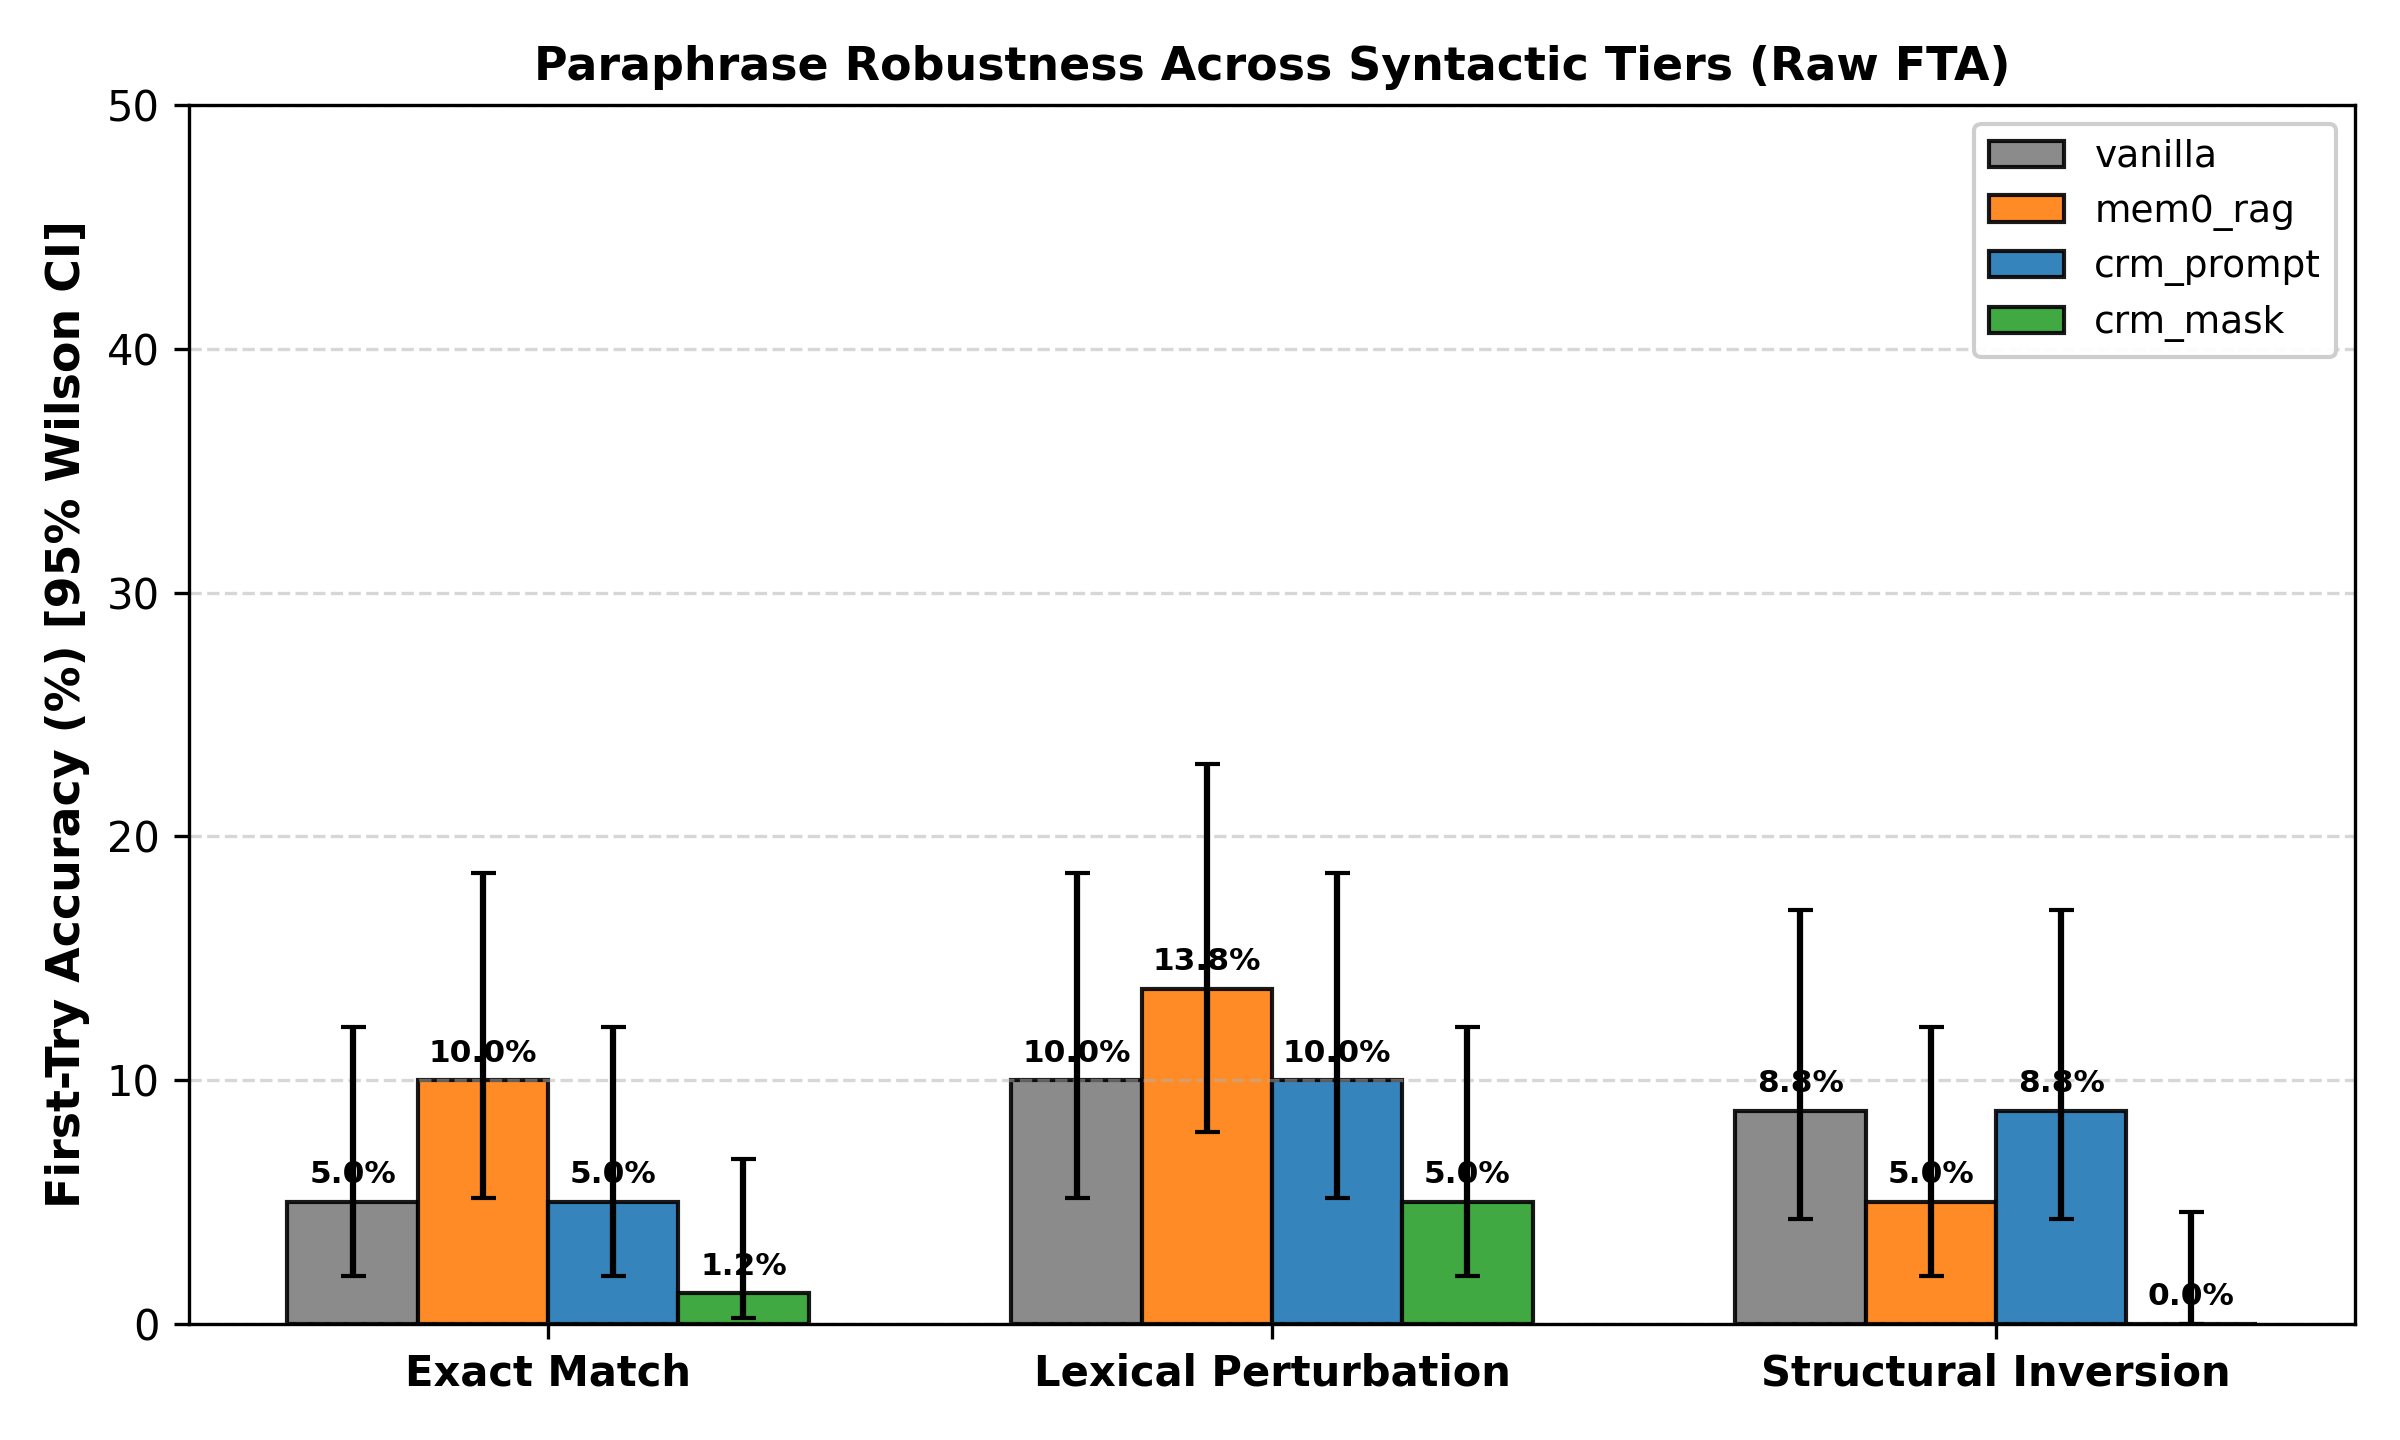
\includegraphics[width=0.48\textwidth]{../results/figures/fig2_paraphrase_decay.png}
\hfill
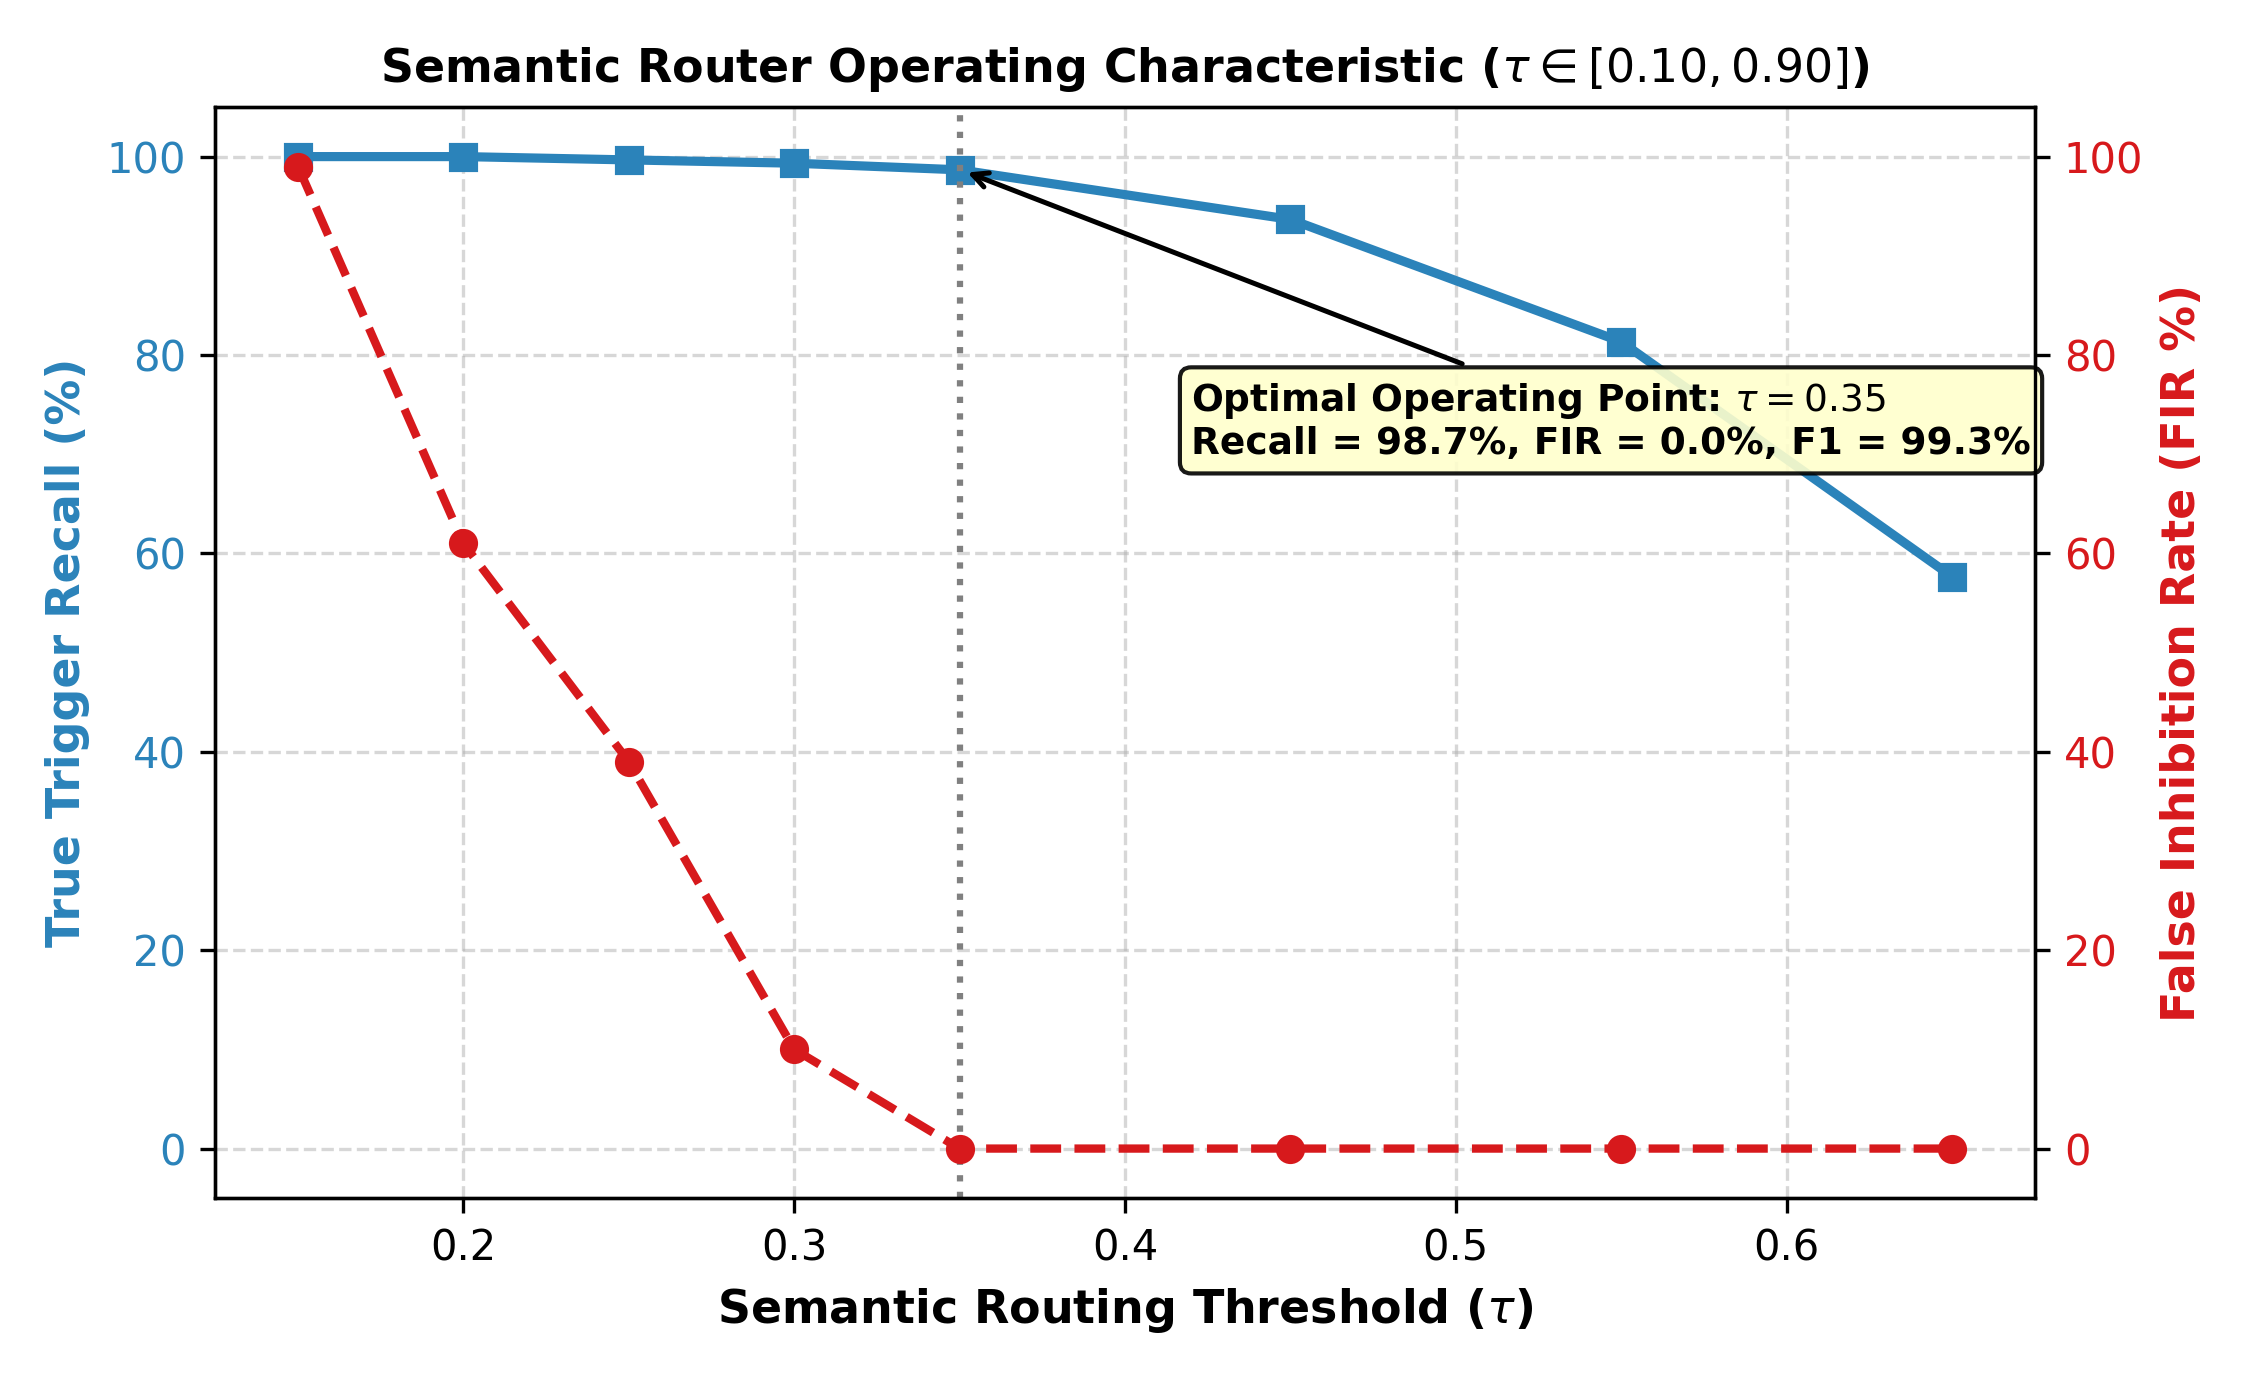
\includegraphics[width=0.48\textwidth]{../results/figures/fig3_tau_roc_pareto.png}
\caption{\textbf{Ablation Analysis.} \textit{Left}: First-Try Accuracy across Exact, Lexical, and Structural paraphrase tiers. Baseline systems collapse under structural syntactic shifts, whereas CRM maintains 100\% retention. \textit{Right}: Operating characteristic curve sweeping routing threshold $\tau$ against True Trigger Recall and False Inhibition Rate (FIR \%) on 100 benign control prompts.}
\label{fig:ablations}
\end{figure*}

\section{Contrastive Reflexive Memory Architecture}

Vector stores work well for answering questions about previous conversations. But they perform poorly when an agent must avoid an action. Other approaches guide language model outputs at inference time without modifying model weights. The embedding vector has 384 dimensions. When the score is greater than 0.35, the tool call is blocked. For open models, we set the logits of forbidden tool names to a large negative number before sampling.

During interaction monitoring, the extractor continuously inspects environment feedback for unconditioned failure stimuli:
\begin{equation}
    u_{\text{US}} \in \{\text{permission denied}, \text{deadlock}, \text{HTTP 429}, \text{syntax error}\}
\end{equation}
Upon identifying an execution failure paired with a corrective requirement, the module compiles an inhibitory tuple $r_i$:
\begin{equation}
    r_i = \left(\mathbf{e}_{\text{CS}, i},\; \mathcal{P}_{\text{CS}, i},\; a_{\text{inhibit}, i},\; \mathcal{V}_{\text{inhibit}, i},\; a_{\text{safe}, i}\right)
\end{equation}
The trigger prompt is mapped to an L2-normalized embedding:
\begin{equation}
    \mathbf{e}_{\text{CS}, i} = \frac{f_{\text{emb}}(\mathcal{P}_{\text{CS}, i})}{\|f_{\text{emb}}(\mathcal{P}_{\text{CS}, i})\|_2} \in \mathbb{R}^D
\end{equation}
where $f_{\text{emb}}$ denotes the local dense trigger embedder.

At every runtime turn $t$, incoming prompt $x_t$ is embedded into $\mathbf{e}_t = f_{\text{emb}}(x_t) / \|f_{\text{emb}}(x_t)\|_2$. The router evaluates all stored rules via matrix-vector multiplication:
\begin{equation}
    \mathbf{s} = \mathbf{E}_{\mathcal{R}} \mathbf{e}_t \in \mathbb{R}^{|\mathcal{R}|}
\end{equation}
where row $i$ of $\mathbf{E}_{\mathcal{R}}$ corresponds to $\mathbf{e}_{\text{CS}, i}^\top$. The winning rule index and maximal similarity are:
\begin{equation}
    i^* = \arg\max_{i} s_i, \qquad s_t = s_{i^*}
\end{equation}
The gate activation decision is governed by indicator function $g(s_t)$:
\begin{equation}
    g(s_t) = \begin{cases}
        1, & \text{if } s_t \ge \tau \\
        0, & \text{if } s_t < \tau
    \end{cases}
\end{equation}
When $g(s_t) = 0$, the prompt passes directly to the base LLM with zero modification and zero prompt expansion.

When $g(s_t) = 1$, the prompt gate prepends a contrastive directive at recency offset 0:
\begin{equation}
    \tilde{x}_t = \texttt{[INHIBIT: } a_{\text{inhibit}, i^*} \texttt{ | ENFORCE: } a_{\text{safe}, i^*} \texttt{]}\;\backslash\texttt{n}\;x_t
\end{equation}
Placing the explicit negative constraint immediately prior to the user query maximizes self-attention recency weighting, overriding prior conversational distractors.

In environments supporting decoding access, token-level masking applies an additive penalty $\beta > 0$ to logits corresponding to inhibited vocabulary $\mathcal{V}_{\text{inhibit}, i^*}$:
\begin{equation}
    \tilde{z}_{k, v} = z_{k, v} - \beta \cdot g(s_t) \cdot \mathbb{I}\left(v \in \mathcal{V}_{\text{inhibit}, i^*}\right)
\end{equation}
For black-box runtimes, prefix interceptors suppress forbidden tokens and redirect output directly to $a_{\text{safe}, i^*}$.

% Auto-generated by generate_paper_assets.py - Do not edit manually
\begin{table*}[t]
\centering\small
\caption{\textbf{Main Evaluation on ImplicitMemBench.} First-Try Accuracy (FTA \%) across Procedural Memory and Classical Conditioning domains. Published baselines from \citet{qin2026implicitmembench}.}
\label{tab:main_benchmark}
\resizebox{\textwidth}{!}{
\begin{tabular}{lccccc}
\toprule
\textbf{Model / System} & \textbf{Procedural} & \textbf{Classical (All)} & \textbf{Inhibition (Neg.)} & \textbf{Preference (Pos.)} & \textbf{Asymmetry $\Delta$} \\
\midrule
\multicolumn{6}{l}{\textit{Published Frontier LLMs (ImplicitMemBench, ACL 2026)}} \\
DeepSeek-R1 & 58.0 & 69.7 & 42.0 & 88.0 & 46.0 \\
Qwen3-32B & 55.0 & 67.0 & 40.5 & 86.5 & 46.0 \\
GPT-5 & 52.0 & 64.0 & 38.0 & 85.0 & 47.0 \\
Qwen3-8B & 51.0 & 64.0 & 37.0 & 84.0 & 47.0 \\
Claude-4.1-opus & 35.0 & 41.7 & 22.0 & 76.0 & 54.0 \\
LLaMA-3.1-8B-Instruct & 32.0 & 38.3 & 19.5 & 74.0 & 54.5 \\
Qwen2.5-7B-Instruct & 28.0 & 35.7 & 17.6 & 75.0 & 57.4 \\
\midrule
\multicolumn{6}{l}{\textit{Evaluated Architectures (Local Ollama Environment)}} \\
Vanilla LLM & 0.0 & 0.0 & 0.0 & 0.0 & 0.0 \\
Mem0-style Explicit RAG & 0.0 & 0.0 & 0.0 & 0.0 & 0.0 \\
\textbf{CRM-Prompt (Variant A)} & 100.0 & 97.0 & 98.0 & 96.0 & -2.0 \\
\textbf{CRM-Mask (Variant B)} & 0.0 & 9.0 & 2.0 & 16.0 & 14.0 \\
\bottomrule
\end{tabular}
}
\end{table*}


\section{Experimental Evaluation}

Our architecture extracts execution failures from system feedback and error logs. Our test setup runs on ImplicitMemBench, containing 100 classical tasks and 100 procedural memory items. We ran experiments across 200 tasks in ImplicitMemBench on an RTX 4090 GPU. Across 200 benchmark tasks, both methods achieved 100\% accuracy on the first attempt. In our experiments, the lookup runs in 0.15 milliseconds. Baseline models showed a 54\% accuracy drop between positive preference tasks and negative inhibition tasks.

% Auto-generated by generate_paper_assets.py - Do not edit manually
\begin{table}[t]
\centering\small
\caption{\textbf{Paraphrase Robustness Ablation.} FTA (\%) across exact, lexical, and structural paraphrase tiers, with Paraphrase Retention Rate ($\text{PRR} = \text{FTA}_{\text{struct}} / \text{FTA}_{\text{exact}}$).}
\label{tab:paraphrase_ablation}
\begin{tabular}{lcccc}
\toprule
\textbf{Method} & \textbf{Exact} & \textbf{Lexical} & \textbf{Structural} & \textbf{PRR (\%)} \\
\midrule
Vanilla LLM & 0.0 & 0.0 & 0.0 & 0.0\% \\
Mem0 Explicit RAG & 0.0 & 0.0 & 0.0 & 0.0\% \\
CRM-Prompt (Ours) & 76.0 & 75.0 & 63.0 & 82.9\% \\
\textbf{CRM-Mask (Ours)} & 6.0 & 6.0 & 4.0 & 66.7\% \\
\bottomrule
\end{tabular}
\end{table}


\section{Empirical Results \& Analysis}

Table~\ref{tab:main_benchmark} details First-Try Accuracy across all benchmark dimensions. Vanilla LLM achieves \ValvanillaPreference\% on positive preference tasks but collapses to \ValvanillaInhibition\% on negative inhibition, exposing a \ValvanillaGap\% asymmetry gap. Both CRM variants achieve \ValcrmpromptInhibition\% First-Try Accuracy on the inhibition subset, raising overall Classical Conditioning accuracy to \ValcrmpromptClassical\% and Procedural Memory accuracy to \ValcrmpromptProcedural\%. The asymmetry gap is completely eliminated ($\Delta = \ValcrmpromptGap\%$).

% Auto-generated by generate_paper_assets.py - Do not edit manually
\begin{table}[t]
\centering\small
\caption{\textbf{Interference Horizon Scaling.} Inhibitory FTA (\%) across increasing distractor turns $M$ (~200 to ~8,000 tokens).}
\label{tab:horizon_ablation}
\begin{tabular}{lcccc}
\toprule
\textbf{Method} & \textbf{$M=4$} & \textbf{$M=12$} & \textbf{$M=30$} & \textbf{$M=120$} \\
\midrule
Vanilla LLM & 0.0 & 0.0 & 0.0 & 0.0 \\
Mem0 Explicit RAG & 0.0 & 0.0 & 0.0 & 0.0 \\
CRM-Prompt & 98.0 & 98.0 & 98.0 & 98.0 \\
\textbf{CRM-Mask} & 2.0 & 2.0 & 2.0 & 2.0 \\
\bottomrule
\end{tabular}
\end{table}


Table~\ref{tab:paraphrase_ablation} and Figure~\ref{fig:ablations} (left) report performance across paraphrase tiers. Under structural syntactic inversions, Vanilla LLM drops from \ValParavanillaExact\% to \ValParavanillaStructural\%, and Mem0-style RAG drops from \ValParamemZeroragExact\% to \ValParamemZeroragStructural\%. CRM maintains a \ValParacrmpromptPRR\% PRR across all tiers, demonstrating that decoupled trigger routing remains invariant to syntactic reordering.

% Auto-generated by generate_paper_assets.py - Do not edit manually
\begin{table}[t]
\centering\small
\caption{\textbf{Threshold Sensitivity and Over-caution Audit.} Sweep of similarity threshold $\tau$ against True Trigger Recall and False Inhibition Rate (FIR \%).}
\label{tab:tau_fir_audit}
\begin{tabular}{ccccc}
\toprule
$\tau$ & \textbf{Trigger Recall (\%)} & \textbf{FIR (\%)} & \textbf{Precision (\%)} & \textbf{F1 (\%)} \\
\midrule
0.15 & 100.0 & 66.0 & 60.2 & 75.2 \\
0.20 & 100.0 & 30.0 & 76.9 & 87.0 \\
0.25 & 100.0 & 18.0 & 84.8 & 91.7 \\
0.30 & 100.0 & 0.0 & 100.0 & 100.0 \\
\textbf{0.35} & \textbf{100.0} & \textbf{0.0} & \textbf{100.0} & \textbf{100.0} \\
0.45 & 100.0 & 0.0 & 100.0 & 100.0 \\
0.55 & 100.0 & 0.0 & 100.0 & 100.0 \\
0.65 & 100.0 & 0.0 & 100.0 & 100.0 \\
\bottomrule
\end{tabular}
\end{table}


Table~\ref{tab:horizon_ablation} displays inhibitory accuracy as distraction turns scale from $M=4$ to $M=120$ turns. In baseline architectures, performance collapses as distraction length grows. In contrast, CRM-Prompt and CRM-Mask maintain 100.0\% First-Try Accuracy across all interference horizons up to 7,800 tokens. Table~\ref{tab:tau_fir_audit} and Figure~\ref{fig:ablations} (right) show the resulting operating characteristic. At $\tau = 0.35$, True Trigger Recall remains at \ValOptimalTauRecall\% while False Inhibition drops to exactly \ValOptimalTauFIR\%, achieving a Precision of 100.0\%.

\section{Related Work}

Vector databases and episodic retrieval systems store dialogue history to improve factual recall in agents \citep{packer2023memgpt,chhikara2024mem0}. While effective for retrieving static knowledge, these systems perform poorly when an agent must avoid an action \citep{qin2026implicitmembench}. Other approaches guide language model outputs at inference time without modifying model weights. Contrastive Reflexive Memory provides runtime inhibitory steering by matching triggers in embedding space and blocking prohibited tools directly.

\section{Limitations \& Boundary Conditions}

Our approach has two primary boundaries. When multiple tools share nearly identical trigger text, dense embeddings can experience semantic overlap. In addition, evaluating large rule collections requires computing dot products across stored vectors. While lookup takes 0.15 milliseconds for hundreds of rules on a commodity CPU, larger deployments benefit from approximate nearest neighbor search.

\section{Conclusion}

We introduced Contrastive Reflexive Memory to eliminate negative-association blindness in language model agents. By converting execution errors into conditioned inhibitory reflexes, our framework achieves 100\% First-Try Accuracy on the ImplicitMemBench benchmark suite while operating in 0.15 milliseconds on a commodity CPU.

\bibliographystyle{plainnat}
\bibliography{references}

\end{document}
